\documentclass[10pt]{beamer}

%%%
% PREAMBLE FOR THIS DOC 
%%%
%https://tex.stackexchange.com/questions/68821/is-it-possible-to-create-a-latex-preamble-header
\usepackage{/Users/miw267/Repos/csci246_spring2025/slides/preambles/beamer_preamble_for_CSCI246}



%%% TRY TO RESHOW TOC AT EACH SECTION START (with current section highlighted)
% Reference: https://tex.stackexchange.com/questions/280436/how-to-highlight-a-specific-section-in-beamer-toc
\newcommand\tocforsect[2]{%
  \begingroup
  \edef\safesection{\thesection}
  \setcounter{section}{#1}
  \tableofcontents[#2,currentsection]
  \setcounter{section}{\safesection}
  \endgroup
}


%%%% HERES HOW TO DO IT CORRECTLY
% FIRST IN .STY FILE, DO
%\usetheme[sectionpage=none]{metropolis}
% THEN AT EACH SECTION DO
%\begin{frame}{Outline}
%  \tableofcontents[currentsection]	
%\end{frame}



%\setbeamertemplate{navigation symbols}{}
%\setbeamertemplate{footline}[frame number]{}


%%%
% DOCUMENT
%%%

\begin{document}

%\maketitle

%% Title page frame
%\begin{frame}
%    \titlepage 
%\end{frame}





\title{01/31/2025: Induction}
\author{CSCI 246: Discrete Structures}
\date{Textbook reference: Ch. 4, Hampkins}

\begin{frame}
    \titlepage 
\end{frame}


\begin{frame}
\footnotesize 

\begin{mygreenbox}[title=Graded Quiz Pickup]
Quizzes are in the front of the room, grouped into four bins (A-G, H-L, M-R, S-Z) by last name. The quizzes are upside down with your last name on the back. Come find yours before, during, or after class.  Only turn the quiz over if it's yours.
\end{mygreenbox} 
\vfill 

\begin{myredbox}[title=Anonymous (Old School) Poll]
When are picking up your quizzes, please 
\begin{enumerate}
\item Find the glass jar in the front of the room
\item Tear off a sheet of paper 	
\item Write the typical number of hours you spend per week doing work for this class (NOT counting attending class) 
\item Put the paper in the jar
\end{enumerate}
\end{myredbox}

\vfill 


\begin{myyellowbox}[title=Today's Agenda]
\begin{itemize}
	\item Reading \& problems quizzes  (10 mins)
	\item Mini-lecture ($\approx$ 15 mins)
	%
	\begin{itemize}
	\footnotesize 
	\item Induction 
	\item Boolean Algebra properties
	\end{itemize}
	%
	\item Group exercises ($\approx$ 20 mins)
\end{itemize}

\end{myyellowbox}
\vfill 

\end{frame}




\begin{frame}{Today's Quiz}

\begin{myyellowbox}[title=Logistics Alert]
Please write your last name on the back of the page. 
\end{myyellowbox}
\vfill


 \begin{myredbox} [title=Problems Quiz (Secs. 5 and 6 - Proofs and Counterexamples)]
Is the sum of two odd numbers always even?  If so, provide a proof. If not, provide a counterexample.
\end{myredbox}


 \begin{mygreenbox}[title=Reading Quiz (Induction)]
Prove that the $n$-th triangular number is $n(n+1)/2$.  That is, prove 
\[1+ 2+ 3+ \cdots + n = n(n+1)/2.\]
\begin{figure}[ht]
 \centering
 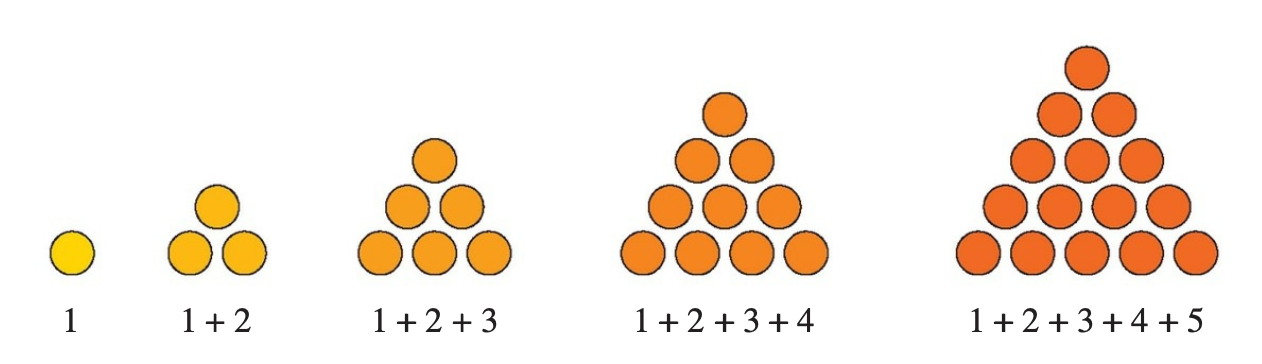
\includegraphics[width=0.6\textwidth]{images/triangular_numbers}
\end{figure}
\end{mygreenbox}

\end{frame}




\begin{frame}{The Induction Strategy to Proving Things}
\small
 \begin{mygreenbox}[title=Reading Quiz (Induction)]
Prove that the $n$-th triangular number is $n(n+1)/2$.  That is, prove 
%
\begin{align*}
1+ 2+ 3+ \cdots + n = n(n+1)/2.
\end{align*}
%
\end{mygreenbox}

\vfill 

 \begin{myyellowbox}[title=Induction Strategy]
\begin{figure}
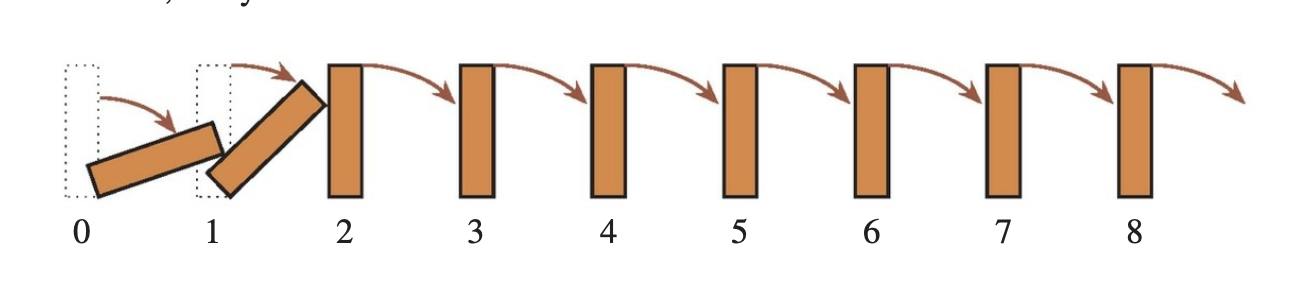
\includegraphics[width=\textwidth]{images/dominos.png}
\end{figure}

\textbf{Base.} Show the equation holds for some starting point (usually 0 or 1).

\textbf{Induction step.} Show that if the equation holds for natural number $n$, then it holds for natural number $n+1$.   
 \end{myyellowbox}

\vfill 
The strategy in the \gold{yellow box} lets us conclude the equation holds for all $n$.
\end{frame} 

\begin{frame}{Solving the Reading Quiz By Induction}
\small
 \begin{mygreenbox}[title=Reading Quiz (Induction)]
Prove that the $n$-th triangular number is $n(n+1)/2$.  That is, prove 
%
\begin{equation}
\bluemathbox{1+ 2+ 3+ \cdots + n} = \bluemathbox{n(n+1)/2}.
\label{eqn:triangular_number_identity}
\end{equation}
\vspace{-0.6cm}
\end{mygreenbox}

\textbf{Base.} We show \Eqref{eqn:triangular_number_identity} holds for $n=1$.  In that case, the RHS of \Eqref{eqn:triangular_number_identity} is
\[ \frac{n(n+1)}{2} = \frac{1(1+1)}{2} = 1, \]
which equals the LHS of \Eqref{eqn:triangular_number_identity}. \\

\textbf{Induction step.}  We show that if the equation holds for some $n$, then it also holds for $n+1$. In other words, we assume \Eqref{eqn:triangular_number_identity}, and we must show
%
 \begin{equation}
\bluemathbox{1+ 2+ 3+ \cdots + n} + n+1 = (n+1)(n+2)/2.
\label{eqn:triangular_number_inductio_step}
\end{equation}
%
We have
%
\begin{align*}
 \text{LHS of \Eqref{eqn:triangular_number_inductio_step}} &= \bluemathbox{\frac{n(n+1)}{2}} \; + \; (n+1) && \scripttext{(by assumption)}\\
 &= \frac{(n+1)(n+2)}{2} && \scripttext{(after some algebra)}	
\end{align*}
\end{frame}

\begin{frame}{Boolean Algebra Properties}
\footnotesize 
\begin{figure}[ht]
        \centering
        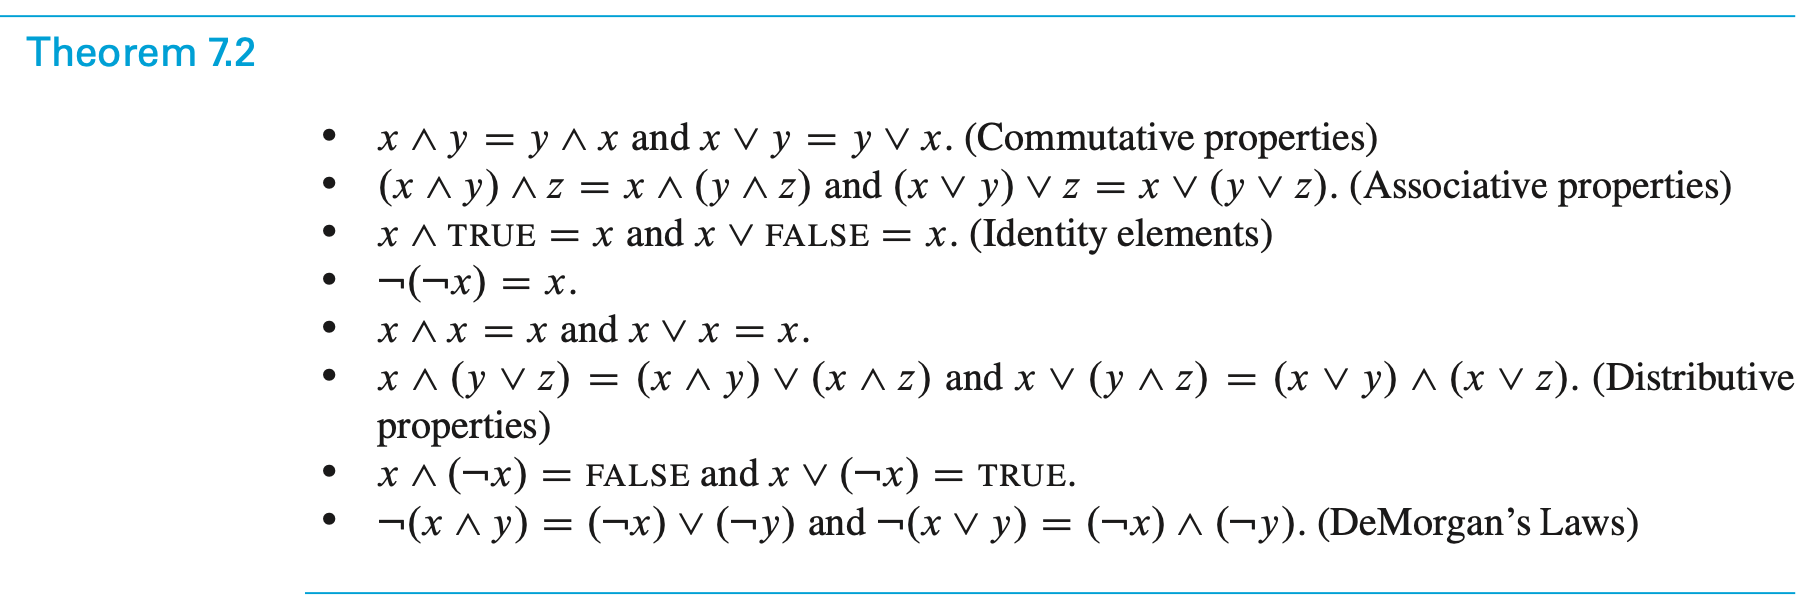
\includegraphics[width=\textwidth]{images/boolean_algebra_properties}
        \caption{Boolean Algebra Properties}
        \label{fig:bap}
\end{figure}

\vfill 

\begin{myredbox}[title=Example application]

We can show that $(x \lor y) \lor (x \lor \lnot y)$ is a tautology as follows
%
\begin{align*}
(x \lor y) \lor (x \lor \lnot y) &= 	(x \lor x) \lor (y \lor \lnot y) && \scripttext{(commutative, associative props.)} \\
&= x \lor \texttt{True} && \scripttext{(unnamed props \#5,7)} \\
&= \texttt{True} && \scripttext{(unnamed prop \#7)}
\end{align*}

instead of using truth tables.
\end{myredbox}	
% Can be faster than writing otu truth tables, especially if many variabels are involved.
\end{frame}



\begin{frame}{Reading Quiz Scoring Rubric: Multiple Proofs}

\begin{myredbox}[title=Scoring rubric (out of 10 points)]
\begin{tabularx}{\textwidth}{|X|L{1cm}|L{1cm}|}
\hline 
\textbf{Description} & \textbf{Main} & \textbf{E.C.} \\
\hline 
Correct and well-written. &10 & 2 \\
 Good work but some mathematical or writing errors that need addressing. &7.5& 1\\
Some good intuition, but there is at least one serious flaw. &5 &0  \\
I don't understand this, but I see that you did work on it. &2.5& 0  \\
No work is evident.	&0&0  \\
\hline
\end{tabularx}
\end{myredbox}
\end{frame}


\begin{frame}{Reading Quiz Scores: Multiple Proofs}

\begin{figure}[ht]
        \centering
        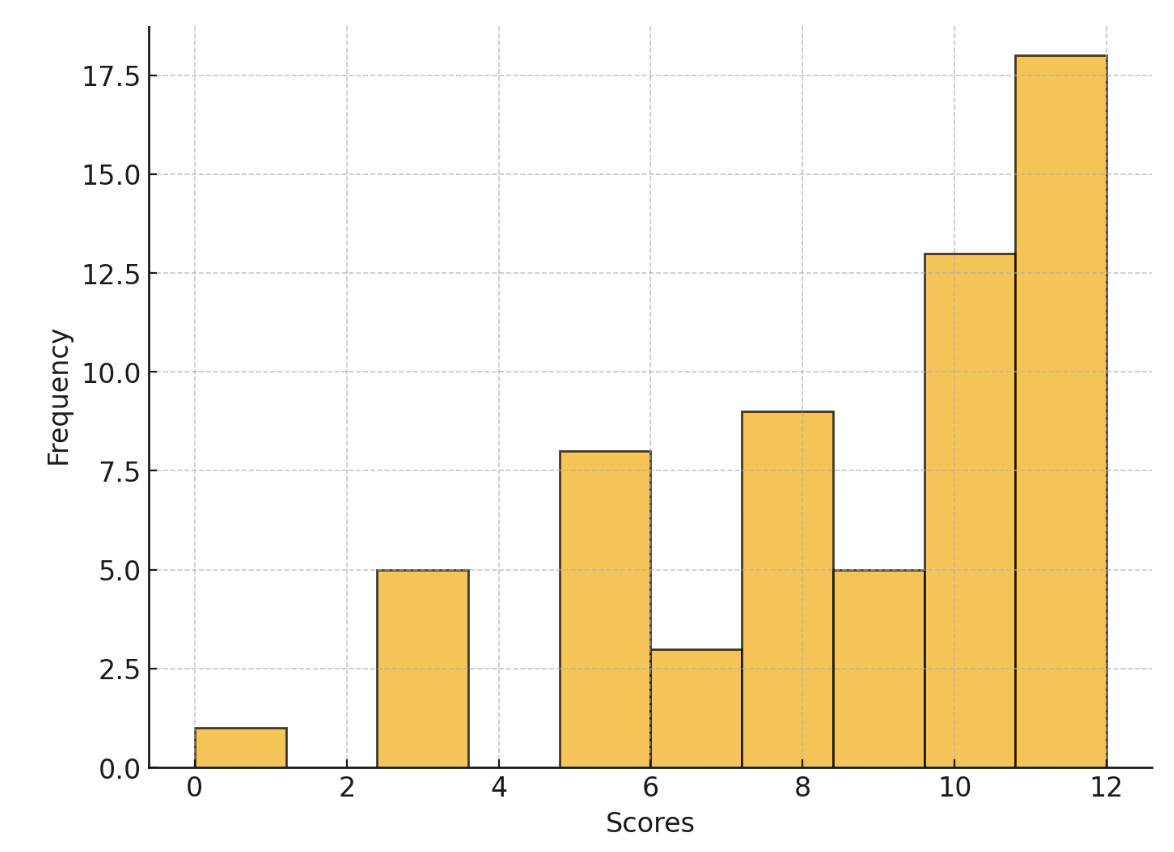
\includegraphics[width=.8\textwidth]{images/ch2_reading_quiz_scores}
        %\caption{Reading Quiz Scores}
        %\label{fig:figure2}
\end{figure}
\vfill 

\end{frame}



\begin{frame}{Factorial notation}

For group work, you will need the definition (really just notation) below. 

\vfill 
\begin{mygreenbox}[title=Definition]
The \textbf{factorial} of a non-negative integer $n$ (denoted by $n!$) is the product of all positive integers less than or equal to $n$. \\

That is,
\[n! \defeq n \times (n-1) \times \cdots \times 2 \times 1.\]
\end{mygreenbox}

\vfill 

\begin{myredbox}[title=Example]
\[ 5! = 5 \times 4 \times 3 \times 2 \times 1 = 120  \]
\end{myredbox}

\vfill 

\begin{myyellowbox}[title=Convention]
By convention, we define 
\[0! =1 \]
\end{myyellowbox}

\end{frame}




\begin{frame}
\footnotesize
Group 1: samuel.hemmen,derek.price4,peter.buckley1\\
Group 2: carver.wambold,blake.leone,evan.schoening\\
Group 3: james.brubaker,cameron.wittrock,jacob.ketola\\
Group 4: evan.barth,anthony.mann,lynsey.read\\
Group 5: joseph.triem,alexander.goetz,connor.mizner\\
Group 6: ryan.barrett2,alexander.knutson,luka.derry\\
Group 7: mason.barnocky,micaylyn.parker,aaron.loomis\\
Group 8: nolan.scott1,matthew.nagel,samuel.mosier\\
Group 9: yebin.wallace,john.fotheringham,ethan.johnson18\\
Group 10: lucas.jones6,jeremiah.mackey,colter.huber\\
Group 11: sarah.periolat,luke.donaldson1,owen.obrien\\
Group 12: tyler.broesel,michael.oswald,erik.moore3\\
Group 13: joseph.mergenthaler,jett.girard,reid.pickert\\
Group 14: jacob.ruiz1,kaden.price,devon.maurer\\
Group 15: pendleton.johnston,julia.larsen,griffin.short\\
Group 16: justice.mosso,bridger.voss,jacob.shepherd1\\
Group 17: caitlin.hermanson,jakob.kominsky,carsten.brooks\\
Group 18: tristan.nogacki,zeke.baumann,connor.graville\\
Group 19: connor.yetter,delaney.rubb,jonas.zeiler\\
Group 20: jack.fry,jada.zorn,samuel.rollins\\
Group 21: william.elder1,timothy.true,peyton.trigg\\
Group 22: adam.wyszynski,emmeri.grooms,conner.reed1
\end{frame}


\begin{frame}{Group exercises: Induction, and finishing up Boolean Algebra}
\footnotesize 

Finish up the Boolean Algebra group exercises (focusing on question \#4).

\vfill 

Also try the following induction problem:

\begin{mygreenbox}
Show by induction that $2^n < n!$ for all $n \geq 4$.
\end{mygreenbox}
\end{frame}


\end{document}
